

\RequirePackage{fix-cm}

\documentclass{svjour3}\usepackage[]{graphicx}\usepackage[]{color}
%% maxwidth is the original width if it is less than linewidth
%% otherwise use linewidth (to make sure the graphics do not exceed the margin)
\makeatletter
\def\maxwidth{ %
  \ifdim\Gin@nat@width>\linewidth
    \linewidth
  \else
    \Gin@nat@width
  \fi
}
\makeatother

\definecolor{fgcolor}{rgb}{0.345, 0.345, 0.345}
\newcommand{\hlnum}[1]{\textcolor[rgb]{0.686,0.059,0.569}{#1}}%
\newcommand{\hlstr}[1]{\textcolor[rgb]{0.192,0.494,0.8}{#1}}%
\newcommand{\hlcom}[1]{\textcolor[rgb]{0.678,0.584,0.686}{\textit{#1}}}%
\newcommand{\hlopt}[1]{\textcolor[rgb]{0,0,0}{#1}}%
\newcommand{\hlstd}[1]{\textcolor[rgb]{0.345,0.345,0.345}{#1}}%
\newcommand{\hlkwa}[1]{\textcolor[rgb]{0.161,0.373,0.58}{\textbf{#1}}}%
\newcommand{\hlkwb}[1]{\textcolor[rgb]{0.69,0.353,0.396}{#1}}%
\newcommand{\hlkwc}[1]{\textcolor[rgb]{0.333,0.667,0.333}{#1}}%
\newcommand{\hlkwd}[1]{\textcolor[rgb]{0.737,0.353,0.396}{\textbf{#1}}}%
\let\hlipl\hlkwb

\usepackage{framed}
\makeatletter
\newenvironment{kframe}{%
 \def\at@end@of@kframe{}%
 \ifinner\ifhmode%
  \def\at@end@of@kframe{\end{minipage}}%
  \begin{minipage}{\columnwidth}%
 \fi\fi%
 \def\FrameCommand##1{\hskip\@totalleftmargin \hskip-\fboxsep
 \colorbox{shadecolor}{##1}\hskip-\fboxsep
     % There is no \\@totalrightmargin, so:
     \hskip-\linewidth \hskip-\@totalleftmargin \hskip\columnwidth}%
 \MakeFramed {\advance\hsize-\width
   \@totalleftmargin\z@ \linewidth\hsize
   \@setminipage}}%
 {\par\unskip\endMakeFramed%
 \at@end@of@kframe}
\makeatother

\definecolor{shadecolor}{rgb}{.97, .97, .97}
\definecolor{messagecolor}{rgb}{0, 0, 0}
\definecolor{warningcolor}{rgb}{1, 0, 1}
\definecolor{errorcolor}{rgb}{1, 0, 0}
\newenvironment{knitrout}{}{} % an empty environment to be redefined in TeX

\usepackage{alltt}                     % onecolumn (standard format)
%\documentclass[smallcondensed]{svjour3}     % onecolumn (ditto)
%\documentclass[smallextended]{svjour3}       % onecolumn (second format)
%\documentclass[twocolumn]{svjour3}          % twocolumn
%

\usepackage{graphicx}
\usepackage{mathptmx}      
\usepackage{amsmath}
\usepackage{graphicx}
\usepackage{booktabs}
\usepackage{multirow}
\usepackage{cite}
\usepackage{caption}
\usepackage{natbib}
\usepackage{longtable}
\usepackage{array}
\usepackage[table]{xcolor}
\usepackage{wrapfig}
\usepackage{float}
\usepackage{colortbl}
\usepackage{pdflscape}
\usepackage{tabu}
% \usepackage{threeparttable}
% \usepackage{threeparttablex}
% \usepackage[normalem]{ulem}
% \usepackage{makecell}

\raggedbottom

\journalname{Sankhya B}
\IfFileExists{upquote.sty}{\usepackage{upquote}}{}
\begin{document}
%\SweaveOpts{concordance=TRUE}



% Predefine some figures
\begin{knitrout}
\definecolor{shadecolor}{rgb}{0.969, 0.969, 0.969}\color{fgcolor}\begin{kframe}


{\ttfamily\noindent\color{warningcolor}{\#\# Warning: package 'dplyr' was built under R version 3.4.3}}

{\ttfamily\noindent\color{warningcolor}{\#\# Warning: package 'kableExtra' was built under R version 3.4.4}}\end{kframe}
\end{knitrout}

































\title{Comparing Different Planned Missingness Designs in Longitudinal Studies}

\author{Josephine Wood \and Gregory J. Matthews \and Jennifer Pellowski \and Ofer Harel}

\institute{J. Wood \and G. J. Matthews
          \at Loyola University Chicago \\
          1032 W. Sheridan Rd.\\
          Chicago IL, 60660 USA\\
          Tel: (773)508-3558
          \and
          O. Harel 
				\at University of Connecticut \\
						215 Glennbrook Rd. Unit 420\\
						Storrs CT, 06269-4120 USA
              Tel: (860)486-6989 \\
		      \email{ofer.harel@uconn.edu}  
					\and
					J. Pellowski
					\at International Health Institute\\ 
					Brown School of Public Health\\
					Department of Psychiatry and Human Behavior\\
					The Warren Alpert Medical School of Brown University.  
}

\date{Received: date / Accepted: date}
% The correct dates will be entered by the editor



\maketitle


\begin{abstract}
Planned Missingness (PM) designs, in which researchers deliberately collect only partial data, have enjoyed a recent growth in popularity. Among other benefits these designs have been proven capable of reducing the study costs and alleviating participant burden. Past research has shown that Split Form PM designs can be effective in simplifying complex surveys while Wave Missingness PM designs act similarly for Longitudinal studies. However, less work has been done to inform how to implement PM structures into studies which incorporate elements of both survey and longitudinal designs. Specifically, in studies where a questionnaire is given to participants at multiple measurement occasions the best way to design missingness is still unclear. To address this deficiency, data in this hybrid format was simulated under both Split Form and Wave Missingness PM structures. Multiple Imputation techniques were applied to estimate a multilevel logistic model in each of the simulations. Estimated parameters were compared to the true values to see which PM design allowed us to best capture the true model. The results of this study indicate that, compared to the Split Form Design, the Wave Missingness design consistently performed less effectively in capturing the multilevel model. Thus, in the context of longitudinal surveys this study recommends the use of Split Form missingness designs, which performs well under a number of different conditions.

\keywords{Planned Missingness \and Split Form \and Multiform \and Wave Missingness \and Multiple Imputation \and Missing Data.}
\end{abstract}

\section{Introduction}
\label{intro}

Often, studies are conducted longitudinally; measuring participants on numerous separate occasions. This allows researchers to observe how a measurement may change over time. In theory, administering a survey once a month would be successful. However, in practice, as surveys become longer and more frequent, participants may begin to provide ingenuine responses or drop out of the study entirely. To combat this issue, researchers may attempt to shorten the survey or decrease the measurement frequency. Merely truncating a survey results in lost information and infrequent administration does not provide a clear picture of participants' evolution over time. In answer to a difficult question, many researchers have turned to planned missingness when designing experiments.

Planned missingness (PM) designs are a type of experimental design in which some of the data is predetermined to be missing. While it may seem counterproductive to deliberately omit data from the collection process, PM designs have been shown to reduce both participant burden \citep{graham2006planned, saris20048} and the costs of a study \citep{graham2001planned}. Moreover, PM designs can actually increase the quality of collected data by increasing the breadth of a study \citep{little2013planned} as well as decreasing the effects of assessment reactivity and rates of unplanned missingness \citep{harel2015designed}. We further note that while PM designs decrease the efficiency of estimators \citep{rhemtulla2016asymptotic}, decreasing the cost per participant may allow researchers to enroll more participants in a study, offsetting some of the efficiency loss. \par

There have been many different incarnations of the PM design, each crafted to best suit the study at hand. For example, PM designs have been used in the study of longitudinal growth curves \citep{graham2001planned, mcardle1997expanding}, business research \citep{shoemaker1973principles}, behavioral studies \citep{harel2015designed}, biostatistics \citep{andres2006partial, wacholder1994partial}, and educational assessments \citep{zeger1997efficient, sirotnik1977incidence}. This paper focuses on two of the simplest and most applicable PM designs; the Split Form design \citep{raghunathan1995split} and the Wave Missingness design \citep{little2013planned} and their application in a longitudinal study utilizing a multi-level regression model, as it lacks coverage in recent literature. While this paper covers these designs in more detail later, broadly speaking, the Split Form design entails measuring fewer points on a single measurement occasion \citep{raghunathan1995split}. The Wave Missingness design, on the other hand, requires missing an entire measurement occasion within a longitudinal study \citep{graham2001planned}. 

The issue we concern ourselves with arises when a longitudinal study requires multiple items to be collected at each measurement occasion. When implementing a multi-level regression model in this situation, we investigate which planned missingess design is more efficient and accurate. Previous research indicates that for the estimation of correlated latent growth curve models use of the three-form PM design, a special case of Split Form designs \citep{raghunathan1995split}, resulted in low bias on parameter estimates or standard error and high efficiency when compared with wave missingness designs \citep{rhemtulla2014planned}. As our model of interest is a mixed effects model, however, we can not be sure that this result will hold. \par 

To answer our question we performed a simulation study from data obtained in longitudinal research on HIV medication adherence and alcohol-interactivity beliefs \citep{pellowski2016alcohol}. For the PM designs mentioned we simulated sample data and then used multiple imputation (MI) \citep{little2014statistical}  techniques to analyze the data. The PM methods were subsequently evaluated through the assessmemt of the average bias, percent bias, mean squared error, coverage rates, confidence interval length, and estimated fraction of missing information (FMI) \citep{little2014statistical} for parameter estimates in a multilevel model. To make the results generalizable, the experiment was repeated under multiple scenarios: increased sample size, low inter-survey correlation, and high time effect. \par

To delineate the remainder of this paper, in Section 2 we go into more depth on the two PM designs previously mentioned and then move into a discussion on the modern Multiple Imputation technique for dealing with missing data. Next, in Section 3 we briefly describe the dataset we worked with and our method of simulation before moving on to the results of our analyses in Section 4 and a discussion in the final section. \par


\section{Designs and Methods}
\label{sec:1}
\subsection{Split Form Design}
\label{sec:1.1}

Split Form missingness designs \citep{raghunathan1995split}, also  known as Multi-Form \citep{little2013planned} or Matrix Sampling designs \citep{thomas2006evaluation}, are aptly named. Instead of giving participants one large survey, researchers create multiple forms, each containing a subset of the full survey's questions. How these subsets are chosen varies. A common form setup is three-form Block Design \citep{graham1996maximizing} in which the full survey is split into four blocks: X, A, B, and C. Each form of the survey includes the X block as well as two of the remaining blocks. A participant is then given a different form each day of the study. Designing the forms in this manner allows researchers to estimate the relationship between any chosen items, regardless of their blocks. For example, this allows the relationship between an item in block A and another in block C to be estimated and examined. \par

An important consideration here is question distribution. The X-block, being included in every form, should contain either the variables of greatest interest or those with the most predictive ability.

Placing central items in the X-block ensures they are always collected and minimizes the efficiency loss of our analyses \citep{thomas2006evaluation}. On the other hand, placing the most predictive variables in the X-block allows Multiple Imputation to more effectively impute missing values from the other blocks \citep{gottschall2012comparison}. Similarly, it is good practice to place variables which are predictive of each other in separate blocks \citep{gottschall2012comparison}. While this approach provides researchers more freedom when forming the surveys, the puzzle of question distribution introduces new concerns. When the question groupings are not obvious, pilot studies may be necessary to determine the predictive potential of and relationships between variables. The cost and burden associated with an item must also be considered when deciding which block to place it in. For example, if a critical item is overly expensive or difficult to obtain we may be better off excluding it from the X-block \citep{little2013planned}. \par

In addition, the number of blocks must be determined. Including more blocks in the design allows further increased missingness \citep{graham2006planned}. While increasing missingness may allow for further reductions in burden and cost, researchers must consider the disadvantages of more blocks. As more blocks are added, the number of possible forms increases. For example, consider two research teams. The first team divides their survey into an X-block and three other blocks of equal size, each containing 25\% of the survey. The second uses an X-block and nine others with 10\% of the items each. If the teams decide that each form will contain the X-block and two of the other blocks, then the second team will have 36 total forms while the first team can proceed with 3. 
%\textbf{This is all assuming that the blocks represent the optimal question grouping. If this is not known, to account for possible relationships and correlation between questions, the teams would need to consider all possible blocks and create forms for every block configuration. For a 7 question survey, with any one question X block and the other 6 split into three blocks, there are 75 possible block configurations. For each configuration, there are 3 possible forms. So, a team would need to consider 225 different forms. Instead of creating 225 distinct forms, a research team can follow a alternative Split Form method.} \par

This is simple in theory, but for traditional paper surveys this is very difficult to execute. Fortunately, recent technological advances have made the use of electronic questionaires more readily accessible. In this environment form randomization can be automated and the creation of numerous unique forms is no longer an issue. This ability allows another method, hereafter referred to as Split Form planned missingness and illustrated in Figure \ref{fig:formillustration}, to be implemented. Split Form is the random exclusion of $k$ questions on a given day, treating each item as its own block \citep{silvia2014planned}.  Using this method, researchers reap the benefits of including all possible variable relationships through increased forms without the difficulty caused by manually building these forms. \par

\subsection{Wave Missingness Design}
\label{sec:1.2}
While Split Form missingness can be applied to many experimental designs, the Wave Missingness design \citep{little2013planned} is unique to studies with multiple measurement occasions, or ``waves". Unlike the Split Form design, where participants miss a subset of items in a single measurement occasion, the Wave Design entails randomizing participants to miss a measurement occasion entirely. An example of a Wave Missing design is shown in Figure \ref{fig:formillustration} where data is collected monthly over the course of 5 months. However, each participant is only measured at three of these occasions. \par

A relative advantage of the Wave Missingness design over the Split form design is increased control over the level of missingness. For studies with many measurement occasions, it is easy to make small changes to the amount of missing data. For example, the data described by \citet{pellowski2016alcohol} records measurements for 45 days. Missing eleven days here would result in 24.4\% missingness while missing twelve gives us 26.7\%. Further, Wave Missingness designs eclipse Split Form designs in terms of cost reduction \citep{little2013planned}. \par

Another advantage of this design is many longitudinal study designs already use the Wave Missingness structure \citep{little2013planned}. Cohort Sequential Designs require cohorts of different ages to be followed longitudinally in such a way that the information from one cohort can be used to impute values for another \citep{little2013longitudinal, duncan2013introduction}. For example, there were three cohorts of ages 10, 11, and 12 at baseline and measured annually for four years. Although measurement only occurs at four waves we can frame this as a six-wave study where the 10-year old cohort has missing values at waves five and six, the 11-year old cohort at waves one and six, and the 12-year old cohort at waves one and two. Because the 10-year old cohort is the only group observed at the first wave, the missing values for the other groups are imputed using this information. By continuing in this manner the data that was collected over a four year period is extended it to cover six years, accelerating the study. The setup of this type of study is demonstrated in Table \ref{tab:cohort}, where "1" and "0" respectively indicate an included and excluded wave. \par

\begin{table}[H]
	\centering
	\caption{Cohort Sequential Design}
	\label{tab:cohort}
	\setlength{\tabcolsep}{0.5cm}
	\begin{tabular}{c|cccccc}
		\toprule
		& \multicolumn{6}{c}{Age} \\
		Participant & 10 & 11 & 12 & 13 & 14 & 15 \\
		\midrule
		1 & 1 & 1 & 1 & 1 & 0 & 0\\
		2 & 0 & 1 & 1 & 1 & 1 & 0\\
		3 & 0 & 0 & 1 & 1 & 1 & 1\\
		\bottomrule
	\end{tabular}
\end{table}

Developmental time-lag models \citep{mcardle1997expanding} use the Wave Missingness structure, as well. As shown in Table \ref{tab:devtimelag}, researchers observe participants at only two measurement occasions, varying the length between occasions for each participant, and then treat this two-time-point data as multi-time-point data with missing values. Under this framework they impute these missing values and estimate growth curve models. Estimating this type of model would normally require measuring participants at many time points. However, under the Wave Missingness design this is accomplished with only two measurement occasions per participant. These designs exemplify how useful the Wave Missingness structure is in accelerating longitudinal studies. \par

\begin{table}[H]
	\centering
	\caption{Developmental Time-Lag Setup}
	\label{tab:devtimelag}
	\setlength{\tabcolsep}{0.75cm}
	\begin{tabular}{c|cccc}
		\toprule
		& \multicolumn{4}{c}{Wave} \\
		Participant & 1 & 2 & 3 & 4 \\
		\midrule
		1 & 1 & 1 & 0 & 0 \\
		2 & 1 & 0 & 1 & 0 \\
		3 & 1 & 0 & 0 & 1 \\
		\bottomrule
	\end{tabular}
\end{table}

\subsection{Altered Split Form}

The Split Form planned missingness method can be modified to include the benefits of complete cases seen in Wave Missingness in what may be called Altered Split Form. In this method, the researcher asks participants all questions on the first $n$ days of the study. Thereafter, the survey design reverts to regular Split Form. This method allows the researcher to collect $n$ complete cases from each participant, aiding in the imputation process after surveys are administered. Altered Split Form, and the other planned missingness methods, is illustrated in Figure \ref{fig:formillustration} below.

\begin{knitrout}
\definecolor{shadecolor}{rgb}{0.969, 0.969, 0.969}\color{fgcolor}\begin{figure}[H]
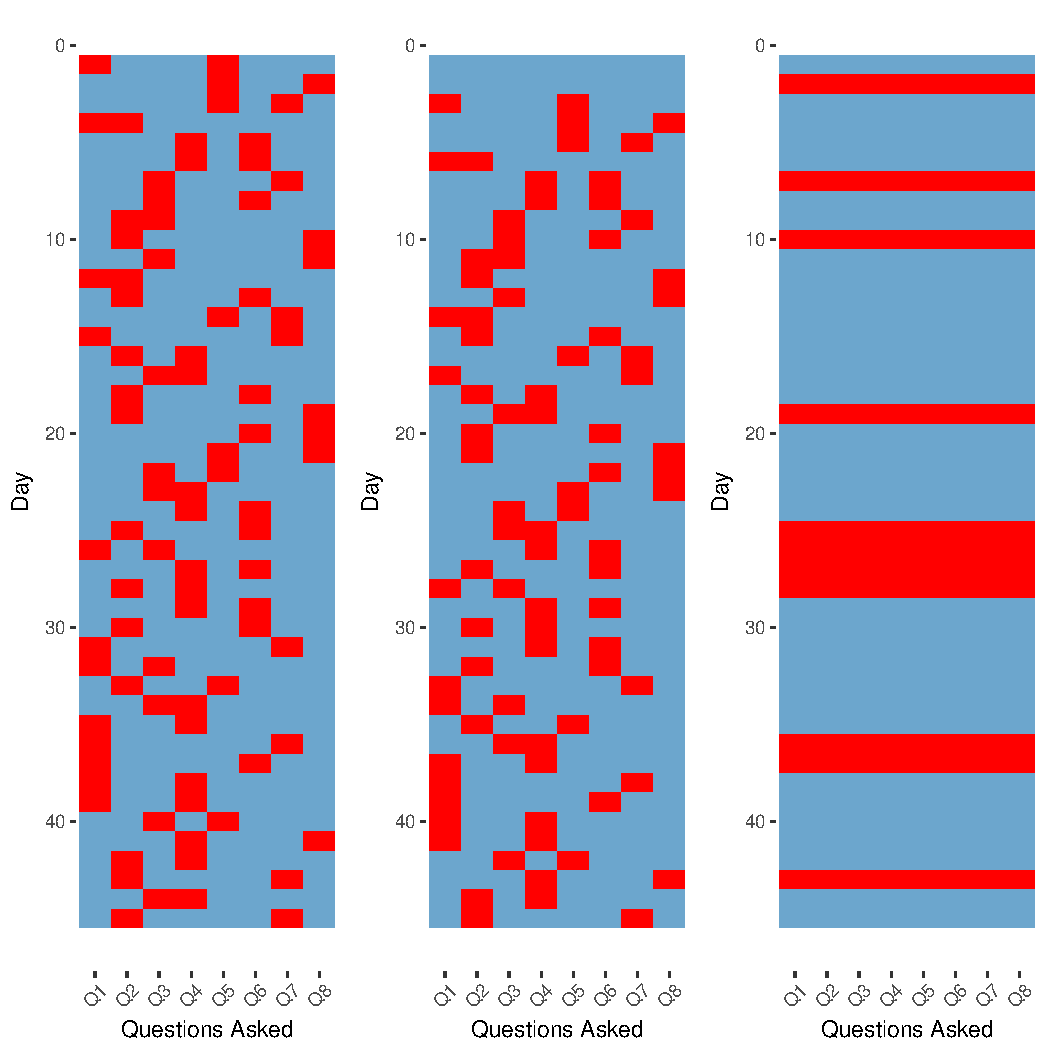
\includegraphics[width=\maxwidth]{figure/formillustration-1} \caption[Low missingness]{Low missingness}\label{fig:formillustration}
\end{figure}


\end{knitrout}

\subsection{Multiple Imputation}
\label{sec:1.3}
\subsubsection{Missing Data Mechanisms}
\label{sec:1.3.1}
Before describing Multiple Imputation and how it can be applied to PM designs it is important to first understand how data become incomplete. Suppose we have a dataset, $Y_{com}$, with some missing values. We define the missingness, $R$, to be an indicator variable which equals 0 where $Y_{com}$ is observed and 1 where the corresponding value in $Y_{com}$ is missing. Missing data mechanisms describe the proposed probabilistic relationship between $R$ and the values in $Y_{com}$, observed or unobserved \citep{little2014statistical}. \par

The first missing data mechanism, missing at random (MAR), was defined by \citet{rubin1976inference}. Data are considered MAR when the missingness does not depend on unobserved values but may depend upon other observed variables. For instance, if men are less likely to report their incomes than women but the level of income itself does not affect the probability of reporting, then we can say the missingness govern income is MAR. \par

Later, \citet{little2014statistical} described two additional mechanisms which lead to missing values: missing completely at random (MCAR) and missing not at random (MNAR) \citep{little2014statistical}. The first, MCAR, is used to describe a situation in which the missingness is independent of the observed or unobserved data. That is, the missing values are simply a random subset of the full data. On the other hand, data is said to be MNAR when the missingness is related to the unobserved data; in a survey people may be less willing to provide their income if it is extremely high or low, for example. \par

If we have prior knowledge concerning the relationship between unobserved values, indicated by $R$, and the observed values, then Multiple Imputation can yield efficient estimates even under MNAR \citep{harel2007multiple}. However, because this is not typically the case, MI is most often implemented under MCAR or MAR assumptions \citep{little2014statistical}. \par

As a consequence of allowing researchers to decide which values in a dataset are observed and unobserved, PM designs grant control over the missing data mechanism. Because of this, MI is an appealing option for researchers utilizing a PM design. If implemented properly, data should conform to either the MCAR or MAR assumption. For instance, if medical researchers decide not to collect blood pressure on a completely random subset of patients there is no reason to believe the missing blood pressures differ significantly from the observed ones. This fact allows for the use of MI and other modern missing data techniques such as the Full Information Maximum Likelihood approach \citep{dempster1977maximum}. \par

\subsubsection{The Multiple Imputation Procedure}
\label{sec:1.3.2}
Multiple Imputation is used to obtain statistically valid inferences in spite of missing data. MI works by replacing unobserved values with a set of plausible values in a way which allows us to account for uncertainty in the imputation process. Repeatedly using an imputation technique, every missing value in the incomplete dataset is replaced with a fixed number of imputed values. This process allows for the creation of multiple complete datasets, on which users can run complete-data procedures. If, for instance, we imputed $M$ possible values for every missing value we would obtain $M$ different completed datasets. Once created, the analysis of interest can be performed on each of them and, using Rubin's rules detailed in \citet{rubin2004multiple}, combine the results to obtain a single inference. \par

Suppose we are interested in estimating a certain parameter such as the mean of a variable or a regression coefficient. If $\theta$ is the parameter of interest, let $\widehat{\theta_1}, \widehat{\theta_2}, ... \widehat{\theta_M}$ be the estimates of $\theta$ and let $S_1, S_2, ... S_M$ be the corresponding estimated standard errors from the $M$ imputed datasets. We can aggregate these results using the combining rules specified in \citet{rubin2004multiple}. \par
The overall MI estimate of $\theta$ is defined as,

\begin{equation}
\widehat{\theta} = \sum_{n=1}^{M} \frac{1}{M} \widehat{\theta_n}.
\end{equation}

From here we can compute the sample variance of this estimate by calculating the between-imputation component, $B_M = \frac{1}{(M-1)}\sum_{n=1}^{M} (\widehat{\theta_n} - \widehat{\theta})^2$, and the within-imputation component, $W_M = \frac{1}{M}\sum_{n=1}^{M} S_n^2$. These components are combined to obtain the overall sample variance of our MI estimate as follows:

\begin{equation}
T_M = W_M + \frac{M+1}{M}B_M.
\end{equation}

These equations form the basis of Rubin's combining rules and provide unbiased parameter estimates accounting for the inherent uncertainty in the imputation process \citep{raghunathan2015missing}. For a more in depth explanation of these methods we refer readers to \citet{little2014statistical}. \par

When using Multiple Imputation, researchers must decide on the number of imputations, $M$, to use. Generally, as the level of missingness decreases the number of imputations needed does as well. \textbf{Greg: IS THIS TRUE?} If less than 20\% of the requisite data are missing, for instance, five or ten imputations will suffice \citep{raghunathan2015missing}. However, at its roots, MI is a simulation technique and thus, the greater $M$ is the more stable our estimates become \citep{harel2007inferences}. \citet{graham2007many} recommend that if computational power is not a limiting factor, then setting $M=100$ is good practice. \par

\section{Data and Simulations}
\label{sec:2}
\subsection{Data}
\label{sec:2.1}
The dataset the simulations are based on originated in a study by \citet{pellowski2016alcohol}. The data was collected in an attempt to determine the day-level relationship between alcohol use, its interactive toxicity beliefs, and adherence to antiretroviral therapy (ART) amongst patients with HIV. Previous studies note that alcohol use combined with the perception that mixing alcohol and ARTs can cause adverse effects, correlated with non-adherence to ARTs \citep{kalichman2009prevalence, kalichman2012alcohol}. However, \citet{pellowski2016alcohol} pointed out that past research collected data over extended periods of time, preventing the identification a day-level interaction. Unlike others, this study was able to determine whether alcohol use and missed medication doses occurred on the same day. \par

The study employed an observational cohort design, following sixty participants over forty-five consequtive days via a daily questionnaire. Questions in the survey concerned livelihood insecurities from the previous day as well as alcohol use. The analysis included eight particular questions: two binary questions on housing insecurity, four binary questions on food insecurity, and two questions concerning alcohol use (one binary variable and one count variable). The exact questions can be found in Table \ref{tab:survey_qs}. \par

\begin{table}[H]
	\centering
	\caption{Survey Questions}
	\label{tab:survey_qs}
	\begin{tabular}{cp{6.5cm}c}
		\toprule
		Item Number & Question & Responses\\
		\midrule
		1 & I worried about having a place to stay yesterday. & 1.Yes $\>$ 2.No \\
		2 & I could not get to where I needed to go yesterday. & 1.Yes $\>$ 2.No \\
		3 & I worried about my food running out yesterday. & 1.Yes $\>$ 2.No \\
		4 & I ate less than I needed to yesterday. & 1.Yes $\>$ 2.No \\
		5 & I was hungry, but did not eat because I couldn't afford food. & 1.Yes $\>$ 2.No \\
		6 & I got food from a pantry, church, agency, friend or the street yesterday. & 1.Yes $\>$ 2.No \\
		7 & Did you drink alcohol yesterday? & 1.Yes $\>$ 2.No \\
		8 & How many alcohol drinks did you have yesterday? & 0-20 \\
		\bottomrule
	\end{tabular}
\end{table}

Beyond the daily questionnaire, data was also collected through a computer-assisted interview on behavioral, psychosocial, and cognitive factors (ex. Income, alcohol-toxicity beliefs, education, etc.) which have been shown to be associated with medication adherence. These values were only collected at baseline and are considered time independent. The variables from this assessment used in our analysis concerned education level, income, age, beliefs about the interactivity of alcohol with ART medication, depression, and alcohol abuse. \par

\subsection{Simulations}
\label{sec:2.2}
The first step in the process of creating the simulated datasets was to obtain parameter estimates from \citet{pellowski2016alcohol} and to quantify the relationships between variables. These estimated relationships were treated as the "true" relationships and one thousand samples were drawn using these parameters. The purpose of simulating these datasets was to see how well they captured the true relationship between daily medication adherence on a certain day, whether or not a participant drank that day, and their beliefs about alcohol-medication interactivity (included as a Z-transformed test score). Specifically, \\

Let $Y_{ij} \sim binomial(n_{ij},p_{ij})$ be whether the $j$th person missed their medication dose on the $i$th day. Then the model of interest is the random intercept model with time effect described as follows:
\begin{align*}
logit(p_{ij}) &= \beta_{0j} + \beta_1DrinkYN_i + \beta_2ZAlcTox_i +\beta_3Day
\end{align*}
where $\beta_{0j} = \gamma_0 + \alpha_j$ and $\alpha_j \sim N(0,\sigma_\alpha^2)$. \\ \\ 
Additionally, note: \\ \\
\begin{itemize}
\item $p_{ij} = 1$ when participant $p$ did not adhere to the ART on day $i$, 0 otherwise \\
\item $DrinkYN = 1$ if participant $p$  drank on day $i$, 0 otherwise\\
\item $ZAlcTox =$ participant $p$'s Z-transformed score on an alcohol-antiretroviral interactive toxicity scale developed by Kalichman \cite{kalichman2009prevalence} \\
\item $Day =$ Day $i$ of the study, 0-44 \\
\item $j =$ participant index, 1-60 \\
\end{itemize}.

Based on the observed data, the true values of the parameters, $\gamma_0$, $\beta_1$, $\beta_2$, $\beta_3$, and $\sigma_\alpha^2$ were found to be -2.29, 0.28, 0.64, 0.01, and 1.12, respectively. \par
Once the samples were drawn, missingness was added under three different structures. These were the Split-Form and Wave Missingness designs previously mentioned as well as a variation on the Split-Form design where a few measurement occasions (here, two days per participant) are fully observed. To clarify this difference, see the hypothetical application of these designs to a five question multi-day survey in Figure \ref{fig:formillustration}. \par


For each different designed missingness pattern we imposed low, medium, and high levels of missingness roughly corresponding to 2, 4, and 6 missing questions. Previous work by \citet{rhemtulla2014planned} found that for low levels of missingness Split Form design outperforms the Wave Missingness design in capturing latent growth curve model parameters. However, because only low-levels of missingness are tested it is unknown whether this relationship holds at moderate or high levels. By including these different levels of missingness the performance at all levels of the missingness spectrum will be measured. \par
Once missingness was created, Multiple Imputation techniques were applied to estimate the relationship between medication adherence and the other variables in our model. Because the missing data mechanism is controled, the data is known to be MCAR. This fact allows for the principled use of MI techniques. Using the R package \texttt{mice} \citep{mice2011imputation} the binary variables (Q1-Q7) were imputed using a logistic model based approach while the count variable (Q8) was imputed using predictive mean matching measure of the proportion of information that is lost as a result of missing data. \par

After imputing, a logistic random-intercept model was estimated for each of the imputed datasets and combined using Rubin's Rules \citep{rubin2004multiple}. From here, the results from each PM design were evaluated based on bias, percent bias, mean squared error (MSE), coverage, confidence interval (CI) length, and the fraction of missing information (FMI). The FMI is a measure of the fraction of information that is lost due to missing data. In addition to comparing the results between each of the PM designs, the same analyses were also performed before missingness was imposed. \par

When determining if the PM designs are performing sufficiently, it is important to consider how well the simulated samples performed before adding a missingness structure. For example, consider two full data samples with respective biases on the $\beta_1$ estimate of 0.13 and 0.15. Further, after imposing different PM design structures on these samples, the average biases are 0.14 and 0.15 respectively. It would be unfair to claim that the first PM design performed better than the second because, by chance, it was based off of a more representative sample. This fact was considered when determining the evaluation criteria. \par

For bias, percent bias, and MSE we claimed that an increase of more than 40\% in these measurements after imposing missingness indicates that the PM design is inappropriate. For instance, if the complete data shows a percent bias of 10\%, anything higher than 14\% would be unacceptable. An increase of this size has the ability to negatively effect efficiency of our estimation. Based on the work of \citet{collins2001comparison} we also regard coverages of less than 90\% as unacceptable. If a 95\% CI has a true coverage of 90\% than the Type I error rate is double what it should be. Because MI accounts for uncertainty in the imputation process, coverages should be similar despite the added missingness. In terms of confidence interval lengths, if one PM design provides similar rates of coverage to another while maintaining shorter intervals than this is considered the better of the two methods. For equal coverage rates, shorter intervals imply more power. The FMI, which quantifies the uncertainty in our imputation process, is simply reported for each PM design. While less uncertainty in the imputations can be beneficial, less variation does not necessarily imply accuracy. Thus, FMI should be taken in the context of the other measurements. \par

This process was repeated under the three modified simulation scenarios mentioned in the following sections. Note that while typically these PM designs would be compared against the results obtained using a complete case analysis \citep{rhemtulla2016asymptotic}, this approach was avoided as it would fundamentally alter the form of the data. Specifically, complete case analysis removes any observation with any missing values. Then, for the Split Form design this would remove all observations. In the Wave Missingness setup, complete case analysis would shorten the length of the longitudinal study. If a participant was missing values on 11 of the 45 days, then complete case analysis would have made the data resemble a longitudinal study held over 34 days. Hence, this comparison is invalid. \par

\subsubsection{Increased Sample Size}
In order to evaluate the impact of sample size on estimation, the original sample size of 60 participants was expanded to 120. The rest of the simulation process was carried out as before. As noted earlier, the cost savings gleaned from the PM designs could allow us to enroll more participants. Thus, even if one design performed more optimally than the others, if all designs also perform acceptably well at high samples, researchers can design missingness in whichever method is most convenient. Furthermore, because Wave Missingness allows for greater savings, an increase in sample size is more reasonable for that type of missingness. \par

\subsubsection{Low Inter-Survey Correlation}
For our second simulation scenario we looked to determine the effect of decreased inter-survey correlation on which PM design would perform best. To clarify, consider the fact that answers given on a particular day may be correlated with one another- the two questions on housing insecurity, for example, are likely to be "yes" on the same days. This set of simulations reduced the correlations between survey questions to study the impact lower correlation between survey question answers.  This was done to simulate a scenario where researchers have a questionnaire that they do not expect any of the answers to be obviously related. To investigate this, the correlation betwen the variables was reduced by half.\par

\subsubsection{High Time Effect}
In the final scenario, the goal was to determine which PM design would lead to the best estimates when time has a disproportionately large effect on our outcome variable. To do this held the values of $\gamma_0$, $\beta_1$, $\beta_2$ the same and increaed the effect of time (i.e. $\beta_3$) by ten times.  The results of this section may prove useful to researchers who believe that the overall passage of time plays a larger role in their outcome than a measurement taken at one specific point. \par

\section{Results}
\label{sec:3}
\subsection{Primary Simulation}
\label{sec:3.1}
The first set of simulations run contained the parameters in the random-intercept logistic model with $\gamma_0 = -2.28$, $\beta_1 = 0.28$, $\beta_2 = 0.64$, and $\beta_3 = 0.01$. The effects of the variables here are comparable to those found in the original dataset. This fact implies that we can interpret the results here to show what may have occurred if the original study had implemented a PM design. Before we imposed a missingness structure on the 1,000 simulated samples we obtained the full data results shown in Table \ref{tab:prelim}. Note that the full data results for the other simulation scenarios are also provided in this table for ease of reference.

\begin{knitrout}
\definecolor{shadecolor}{rgb}{0.969, 0.969, 0.969}\color{fgcolor}\begin{table}[!h]

\caption{\label{tab:unnamed-chunk-2}\label{tab:prelim} Preliminary Results (N = 60)}
\centering
\resizebox{\linewidth}{!}{\begin{tabular}[t]{l|l|r|l|r|l|r}
\hline
Scenario & Parameter & Bias & Pct Bias & MSE & Coverage & CI Length\\
\hline
 & $\gamma_0$ (-2.287) & 0.042 & -1.86\% & 0.018 & 98.8\% & 0.700\\

 & $\beta_1$ (0.282) & -0.103 & -36.45\% & 0.871 & 95.4\% & 3.040\\

 & $\beta_2$ (0.637) & 0.008 & 1.26\% & 0.024 & 93.4\% & 0.585\\

\multirow{-4}{*}{\raggedright\arraybackslash Primary Analysis (n = 60)} & $\beta_3$ (0.0147) & 0.000 & -0.83\% & 0.000 & 94.2\% & 0.017\\
\cline{1-7}
 & $\gamma_0$ (-2.287) & 0.014 & -0.59\% & 0.008 & 98.4\% & 0.424\\

 & $\beta_1$ (0.282) & -0.038 & -13.5\% & 0.135 & 95.2\% & 1.384\\

 & $\beta_2$ (0.637) & 0.006 & 0.86\% & 0.007 & 94.4\% & 0.319\\

\multirow{-4}{*}{\raggedright\arraybackslash Increased Sample Size (n = 120)} & $\beta_3$ (0.0147) & 0.000 & -0.87\% & 0.000 & 95.3\% & 0.012\\
\cline{1-7}
 & $\gamma_0$ (-2.287) & 0.044 & -1.91\% & 0.018 & 98.8\% & 0.700\\

 & $\beta_1$ (0.282) & -0.067 & -23.67\% & 0.298 & 95.8\% & 2.001\\

 & $\beta_2$ (0.637) & 0.007 & 1.11\% & 0.024 & 93.5\% & 0.585\\

\multirow{-4}{*}{\raggedright\arraybackslash Low Inter-Survey Correlation (n = 60)} & $\beta_3$ (0.0147) & 0.000 & -1.17\% & 0.000 & 94\% & 0.017\\
\cline{1-7}
 & $\gamma_0$ (-2.287) & -0.020 & 0.44\% & 0.114 & 96.2\% & 1.368\\

 & $\beta_1$ (0.282) & -6.781 & -4815.84\% & 136.550 & 96.6\% & 88815.966\\

 & $\beta_2$ (0.637) & 0.014 & 4.54\% & 0.047 & 95.7\% & 0.832\\

\multirow{-4}{*}{\raggedright\arraybackslash High Time Effect (n = 60)} & $\beta_3$ (0.147) & 0.000 & -0.98\% & 0.000 & 94.5\% & 0.039\\
\hline
\end{tabular}}
\end{table}


\end{knitrout}

Of note in the complete-data primary analysis is that the coverage of the 95\% CIs is larger than expected for the parameter estimates and the percent bias for the $\beta_1$ estimate is somewhat large. This increased bias is likely due to the difficulties inherent in estimating logistic regression models with rare event data \citep{king2001logistic}. Nevertheless, this must be kept in mind when analyzing the results from the PM designs provided in Table \ref{tab:primary}.

\begin{knitrout}
\definecolor{shadecolor}{rgb}{0.969, 0.969, 0.969}\color{fgcolor}\begin{table}[!h]

\caption{\label{tab:primary}\label{} Primary Results (N = 60)}
\centering
\resizebox{\linewidth}{!}{\begin{tabular}[t]{l|l|l|r|l|r|l|r|r}
\hline
Design & Level & Parameter & Bias & Pct Bias & MSE & Coverage & CI Length & FMI\\
\hline
 &  & $\gamma_0$ & 0.042 & -1.82\% & 0.018 & 98.8\% & 0.702 & 0.002\\

 &  & $\beta_1$ & -0.071 & -25.12\% & 0.269 & 98.3\% & 2.534 & 0.236\\

 &  & $\beta_2$ & 0.008 & 1.25\% & 0.024 & 93.2\% & 0.585 & 0.000\\

 & \multirow{-4}{*}{\raggedright\arraybackslash Low} & $\beta_3$ & 0.000 & -0.89\% & 0.000 & 94.4\% & 0.017 & 0.001\\

 &  & $\gamma_0$ & 0.039 & -1.68\% & 0.018 & 99\% & 0.709 & 0.011\\

 &  & $\beta_1$ & -0.102 & -36.19\% & 0.271 & 99.8\% & 3.500 & 0.534\\

 &  & $\beta_2$ & 0.008 & 1.21\% & 0.024 & 93.3\% & 0.586 & 0.002\\

 & \multirow{-4}{*}{\raggedright\arraybackslash Medium} & $\beta_3$ & 0.000 & -0.42\% & 0.000 & 94.6\% & 0.017 & 0.007\\

 &  & $\gamma_0$ & 0.028 & -1.24\% & 0.027 & 98.5\% & 0.791 & 0.030\\

 &  & $\beta_1$ & -0.107 & -38.05\% & 0.418 & 98.8\% & 4.268 & 0.630\\

 &  & $\beta_2$ & 0.012 & 1.87\% & 0.027 & 93.2\% & 0.613 & 0.005\\

\multirow{-12}{*}{\raggedright\arraybackslash Split Form} & \multirow{-4}{*}{\raggedright\arraybackslash High} & $\beta_3$ & 0.000 & -0.47\% & 0.000 & 94.6\% & 0.020 & 0.020\\
\cline{1-9}
 &  & $\gamma_0$ & 0.042 & -1.83\% & 0.018 & 99\% & 0.701 & 0.001\\

 &  & $\beta_1$ & -0.069 & -24.4\% & 0.283 & 98.3\% & 2.508 & 0.218\\

 &  & $\beta_2$ & 0.008 & 1.27\% & 0.024 & 93.3\% & 0.585 & 0.000\\

 & \multirow{-4}{*}{\raggedright\arraybackslash Low} & $\beta_3$ & 0.000 & -0.95\% & 0.000 & 94.4\% & 0.017 & 0.001\\

 &  & $\gamma_0$ & 0.040 & -1.76\% & 0.018 & 98.8\% & 0.704 & 0.007\\

 &  & $\beta_1$ & -0.117 & -41.57\% & 0.277 & 99\% & 3.385 & 0.508\\

 &  & $\beta_2$ & 0.008 & 1.29\% & 0.024 & 93.1\% & 0.585 & 0.002\\

 & \multirow{-4}{*}{\raggedright\arraybackslash Medium} & $\beta_3$ & 0.000 & -0.99\% & 0.000 & 94.5\% & 0.017 & 0.005\\

 &  & $\gamma_0$ & 0.036 & -1.59\% & 0.021 & 98.9\% & 0.742 & 0.022\\

 &  & $\beta_1$ & -0.158 & -56.11\% & 0.394 & 99.2\% & 4.336 & 0.662\\

 &  & $\beta_2$ & 0.012 & 1.81\% & 0.026 & 93.4\% & 0.601 & 0.006\\

\multirow{-12}{*}{\raggedright\arraybackslash Altered Split Form} & \multirow{-4}{*}{\raggedright\arraybackslash High} & $\beta_3$ & 0.000 & -1.49\% & 0.000 & 94.1\% & 0.018 & 0.021\\
\cline{1-9}
 &  & $\gamma_0$ & 0.040 & -1.76\% & 0.018 & 98.8\% & 0.703 & 0.005\\

 &  & $\beta_1$ & -0.094 & -33.42\% & 0.238 & 99.3\% & 2.995 & 0.433\\

 &  & $\beta_2$ & 0.008 & 1.25\% & 0.024 & 93.4\% & 0.585 & 0.001\\

 & \multirow{-4}{*}{\raggedright\arraybackslash Low} & $\beta_3$ & 0.000 & -0.88\% & 0.000 & 94.3\% & 0.017 & 0.002\\

 &  & $\gamma_0$ & 0.028 & -1.22\% & 0.018 & 99.5\% & 0.744 & 0.051\\

 &  & $\beta_1$ & -0.088 & -31.12\% & 0.240 & 99.2\% & 3.497 & 0.718\\

 &  & $\beta_2$ & 0.009 & 1.44\% & 0.024 & 93.3\% & 0.588 & 0.006\\

 & \multirow{-4}{*}{\raggedright\arraybackslash Medium} & $\beta_3$ & 0.000 & -1.33\% & 0.000 & 94.6\% & 0.017 & 0.025\\

 &  & $\gamma_0$ & -0.004 & 0.19\% & 0.020 & 99.5\% & 0.962 & 0.224\\

 &  & $\beta_1$ & -0.080 & -28.26\% & 0.234 & 98.5\% & 3.791 & 0.886\\

 &  & $\beta_2$ & 0.011 & 1.7\% & 0.024 & 93.8\% & 0.607 & 0.032\\

\multirow{-12}{*}{\raggedright\arraybackslash Wave Missingness} & \multirow{-4}{*}{\raggedright\arraybackslash High} & $\beta_3$ & 0.000 & -3.3\% & 0.000 & 97\% & 0.020 & 0.148\\
\hline
\end{tabular}}
\end{table}


\end{knitrout}

For the Split Form and Altered Split Form designs seen in Table \ref{tab:primary}, note that the greatest loss in efficiency was on the $\beta_1$ estimate. While the CI coverage remained high at all levels of missingness for the two designs, the bias, percent bias, and MSE reached unacceptable levels at the high missingness level. We also point out that the Altered Split Form design did not perform significantly better than the regular Split Form design. While some individual measurements outperformed those from the Split Form design, bias on $\beta_1$ for example, it underperformed in others, such as percent bias on $\beta_3$. In reference to the FMI on the $\beta_1$ estimate, we can see that at low and medium missingness both Split Form designs performed well. That is, there was less variance in the results from th imputed datasets than we expected given the amount of missing data.\par

Towards the bottom of Table \ref{tab:primary}, the Wave Missingness design provided unacceptable results on bias, percent bias, and MSE for the $\beta_1$ estimate at both medium and high levels of missingness. Moreover, at high levels of missingness coverage became unacceptable as coverage probabilities of the 95\% CIs dropped to 88.5\%.  Additionally, we see that CI length for the $\beta_1$ estimate was roughly equal across all designs, despite the fact that the Wave Missingness design provided more biased estimates. \par

\subsection{Increased Sample Size}
\label{sec:3.2}
In the next simulation scenario the sample size was increased to 120 participants. All parameter values were held the same as in the original simulation. Table \ref{tab:prelim}, again, contains the results of the analysis before applying any PM design. The results of the full-data simulations are compared to those obtained from the PM designs, shown in Table \ref{tab:sampsize}. \par

\begin{knitrout}
\definecolor{shadecolor}{rgb}{0.969, 0.969, 0.969}\color{fgcolor}\begin{table}[!h]

\caption{\label{tab:sampsize}Increased Sample Size Results (N = 120)}
\centering
\resizebox{\linewidth}{!}{\begin{tabular}[t]{l|l|l|r|l|r|l|r|r}
\hline
Design & Level & Parameter & Bias & Pct Bias & MSE & Coverage & CI Length & FMI\\
\hline
 &  & $\gamma_0$ & 0.013 & -0.58\% & 0.008 & 98.5\% & 0.424 & 0.001\\

 &  & $\beta_1$ & -0.041 & -14.63\% & 0.134 & 97.5\% & 1.690 & 0.183\\

 &  & $\beta_2$ & 0.006 & 0.87\% & 0.007 & 94.4\% & 0.319 & 0.000\\

 & \multirow{-4}{*}{\raggedright\arraybackslash Low} & $\beta_3$ & 0.000 & -0.87\% & 0.000 & 95.4\% & 0.012 & 0.000\\

 &  & $\gamma_0$ & 0.012 & -0.54\% & 0.008 & 98.5\% & 0.429 & 0.009\\

 &  & $\beta_1$ & -0.073 & -25.97\% & 0.148 & 99.1\% & 2.366 & 0.449\\

 &  & $\beta_2$ & 0.006 & 0.88\% & 0.007 & 94.4\% & 0.320 & 0.002\\

 & \multirow{-4}{*}{\raggedright\arraybackslash Medium} & $\beta_3$ & 0.000 & -0.83\% & 0.000 & 95.3\% & 0.012 & 0.002\\

 &  & $\gamma_0$ & 0.004 & -0.18\% & 0.011 & 97.3\% & 0.465 & 0.025\\

 &  & $\beta_1$ & -0.145 & -51.62\% & 0.304 & 98.3\% & 3.281 & 0.649\\

 &  & $\beta_2$ & 0.007 & 1.14\% & 0.008 & 93.9\% & 0.332 & 0.005\\

\multirow{-12}{*}{\raggedright\arraybackslash Split Form} & \multirow{-4}{*}{\raggedright\arraybackslash High} & $\beta_3$ & 0.000 & 0.24\% & 0.000 & 94.4\% & 0.013 & 0.010\\
\cline{1-9}
 &  & $\gamma_0$ & 0.013 & -0.58\% & 0.008 & 98.4\% & 0.425 & 0.002\\

 &  & $\beta_1$ & -0.032 & -11.19\% & 0.129 & 98\% & 1.677 & 0.173\\

 &  & $\beta_2$ & 0.006 & 0.88\% & 0.007 & 94.4\% & 0.319 & 0.000\\

 & \multirow{-4}{*}{\raggedright\arraybackslash Low} & $\beta_3$ & 0.000 & -0.88\% & 0.000 & 95.2\% & 0.012 & 0.000\\

 &  & $\gamma_0$ & 0.013 & -0.55\% & 0.008 & 98.3\% & 0.426 & 0.005\\

 &  & $\beta_1$ & -0.058 & -20.67\% & 0.145 & 99.6\% & 2.250 & 0.414\\

 &  & $\beta_2$ & 0.006 & 0.88\% & 0.007 & 94.4\% & 0.319 & 0.001\\

 & \multirow{-4}{*}{\raggedright\arraybackslash Medium} & $\beta_3$ & 0.000 & -0.92\% & 0.000 & 95.1\% & 0.012 & 0.002\\

 &  & $\gamma_0$ & 0.011 & -0.46\% & 0.008 & 98.6\% & 0.434 & 0.017\\

 &  & $\beta_1$ & -0.112 & -39.8\% & 0.228 & 99.4\% & 3.245 & 0.691\\

 &  & $\beta_2$ & 0.006 & 0.89\% & 0.007 & 94\% & 0.321 & 0.004\\

\multirow{-12}{*}{\raggedright\arraybackslash Altered Split Form} & \multirow{-4}{*}{\raggedright\arraybackslash High} & $\beta_3$ & 0.000 & -1.05\% & 0.000 & 95.2\% & 0.012 & 0.009\\
\cline{1-9}
 &  & $\gamma_0$ & 0.013 & -0.57\% & 0.008 & 98.5\% & 0.426 & 0.004\\

 &  & $\beta_1$ & -0.064 & -22.79\% & 0.137 & 98.7\% & 2.064 & 0.342\\

 &  & $\beta_2$ & 0.005 & 0.83\% & 0.007 & 94.4\% & 0.319 & 0.001\\

 & \multirow{-4}{*}{\raggedright\arraybackslash Low} & $\beta_3$ & 0.000 & -0.91\% & 0.000 & 95.2\% & 0.012 & 0.001\\

 &  & $\gamma_0$ & 0.010 & -0.45\% & 0.008 & 98.4\% & 0.435 & 0.023\\

 &  & $\beta_1$ & -0.082 & -29.03\% & 0.184 & 99.4\% & 2.979 & 0.630\\

 &  & $\beta_2$ & 0.006 & 0.89\% & 0.007 & 94.3\% & 0.320 & 0.004\\

 & \multirow{-4}{*}{\raggedright\arraybackslash Medium} & $\beta_3$ & 0.000 & -0.96\% & 0.000 & 95.4\% & 0.012 & 0.008\\

 &  & $\gamma_0$ & -0.010 & 0.43\% & 0.010 & 98.8\% & 0.554 & 0.179\\

 &  & $\beta_1$ & -0.059 & -21.09\% & 0.297 & 97\% & 3.760 & 0.859\\

 &  & $\beta_2$ & 0.008 & 1.2\% & 0.007 & 95.2\% & 0.334 & 0.040\\

\multirow{-12}{*}{\raggedright\arraybackslash Wave Missingness} & \multirow{-4}{*}{\raggedright\arraybackslash High} & $\beta_3$ & 0.000 & -2.43\% & 0.000 & 95.5\% & 0.014 & 0.105\\
\hline
\end{tabular}}
\end{table}


\end{knitrout}

First notice the bias of all parameters is lower than in the smaller sample size simulations. Next, the Split Form design performed similarly well as in the first. At low levels of missingness it gave acceptable results for bias, percent bias, and MSE for the $\beta_1$ and for medium levels only the MSE was unacceptable. However, the CI length is relatively far from the complete-data measurement in Table \ref{tab:prelim}. The CI length from the complete-data simulations was 1.384 while at high levels of missingness the CI length reaches 3.281. However, the percent bias on the $\beta_1$ estimate is seriously different from that obtained in the small sample scenario. For example, at medium levels of missingness the percent bias on $\beta_1$ is -25.97\% while for the smaller sample it was -36.19\%.
Similarly to the Split Form design, the Altered Split Form Design also provided unacceptable results for the MSE of the $\beta_1$ estimate at medium missingness and unacceptable bias, percent bias, and MSE at high levels.  \par
For the Wave Missingness design we continue to see the issues observed in the small sample simulations. That is, for the $\beta_1$ estimate the measurements at medium and high levels of missingness are unacceptable and a steep drop off in coverage probability occurs for the 95\% CIs. In fact, at medium and high levels of missingness the coverages remain steady at 99.4\% and 97\%. The $\gamma_0$ parameter also continues to be estimated poorly at high levels of missing data under the Wave Missingness design. \par


\subsection{Low Inter-Survey Correlation}
\label{sec:3.3}
For the next set of simulations sample size returned to 60 participants but the level of inter-survey correlation decreased. The results obtained from the full data simulations are provided in Table \ref{tab:prelim} while the results from the PM designs are given in Table \ref{tab:lowcorr}. \par

\begin{knitrout}
\definecolor{shadecolor}{rgb}{0.969, 0.969, 0.969}\color{fgcolor}\begin{table}[!h]

\caption{\label{tab:lowcorr}Low Inter-Survey Correlation Results (N = 60)}
\centering
\resizebox{\linewidth}{!}{\begin{tabular}[t]{l|l|l|r|l|r|l|r|r}
\hline
Design & Level & Parameter & Bias & Pct Bias & MSE & Coverage & CI Length & FMI\\
\hline
 &  & $\gamma_0$ & 0.042 & -1.86\% & 0.018 & 99\% & 0.702 & 0.002\\

 &  & $\beta_1$ & -0.067 & -23.96\% & 0.265 & 98.1\% & 2.537 & 0.230\\

 &  & $\beta_2$ & 0.007 & 1.12\% & 0.024 & 93.8\% & 0.585 & 0.000\\

 & \multirow{-4}{*}{\raggedright\arraybackslash Low} & $\beta_3$ & 0.000 & -1.11\% & 0.000 & 94\% & 0.017 & 0.001\\

 &  & $\gamma_0$ & 0.041 & -1.77\% & 0.018 & 99.2\% & 0.708 & 0.010\\

 &  & $\beta_1$ & -0.103 & -36.65\% & 0.281 & 99.1\% & 3.492 & 0.535\\

 &  & $\beta_2$ & 0.008 & 1.18\% & 0.024 & 93.4\% & 0.586 & 0.002\\

 & \multirow{-4}{*}{\raggedright\arraybackslash Medium} & $\beta_3$ & 0.000 & -1.03\% & 0.000 & 93.9\% & 0.017 & 0.006\\

 &  & $\gamma_0$ & 0.034 & -1.49\% & 0.026 & 99\% & 0.794 & 0.030\\

 &  & $\beta_1$ & -0.148 & -52.48\% & 0.425 & 99.1\% & 4.285 & 0.621\\

 &  & $\beta_2$ & 0.011 & 1.79\% & 0.028 & 93.5\% & 0.613 & 0.005\\

\multirow{-12}{*}{\raggedright\arraybackslash Split Form} & \multirow{-4}{*}{\raggedright\arraybackslash High} & $\beta_3$ & 0.000 & -0.87\% & 0.000 & 94.1\% & 0.020 & 0.020\\
\cline{1-9}
 &  & $\gamma_0$ & 0.043 & -1.87\% & 0.018 & 98.9\% & 0.701 & 0.001\\

 &  & $\beta_1$ & -0.066 & -23.57\% & 0.258 & 98.4\% & 2.535 & 0.224\\

 &  & $\beta_2$ & 0.007 & 1.12\% & 0.024 & 93.5\% & 0.585 & 0.000\\

 & \multirow{-4}{*}{\raggedright\arraybackslash Low} & $\beta_3$ & 0.000 & -1.2\% & 0.000 & 93.9\% & 0.017 & 0.001\\

 &  & $\gamma_0$ & 0.041 & -1.78\% & 0.018 & 98.8\% & 0.706 & 0.009\\

 &  & $\beta_1$ & -0.096 & -33.99\% & 0.262 & 99.1\% & 3.394 & 0.511\\

 &  & $\beta_2$ & 0.008 & 1.23\% & 0.024 & 93.4\% & 0.585 & 0.002\\

 & \multirow{-4}{*}{\raggedright\arraybackslash Medium} & $\beta_3$ & 0.000 & -1.15\% & 0.000 & 94\% & 0.017 & 0.005\\

 &  & $\gamma_0$ & 0.036 & -1.57\% & 0.020 & 98.6\% & 0.738 & 0.023\\

 &  & $\beta_1$ & -0.174 & -61.69\% & 0.380 & 99.1\% & 4.350 & 0.669\\

 &  & $\beta_2$ & 0.010 & 1.64\% & 0.025 & 93.7\% & 0.598 & 0.005\\

\multirow{-12}{*}{\raggedright\arraybackslash Altered Split Form} & \multirow{-4}{*}{\raggedright\arraybackslash High} & $\beta_3$ & 0.000 & -0.96\% & 0.000 & 94.9\% & 0.018 & 0.024\\
\cline{1-9}
 &  & $\gamma_0$ & 0.041 & -1.79\% & 0.018 & 98.9\% & 0.703 & 0.005\\

 &  & $\beta_1$ & -0.084 & -29.81\% & 0.242 & 99.4\% & 2.967 & 0.423\\

 &  & $\beta_2$ & 0.007 & 1.14\% & 0.024 & 93.6\% & 0.585 & 0.001\\

 & \multirow{-4}{*}{\raggedright\arraybackslash Low} & $\beta_3$ & 0.000 & -1.1\% & 0.000 & 94\% & 0.017 & 0.002\\

 &  & $\gamma_0$ & 0.031 & -1.35\% & 0.018 & 99.2\% & 0.739 & 0.046\\

 &  & $\beta_1$ & -0.112 & -39.82\% & 0.246 & 98.8\% & 3.491 & 0.722\\

 &  & $\beta_2$ & 0.008 & 1.27\% & 0.024 & 93.6\% & 0.588 & 0.005\\

 & \multirow{-4}{*}{\raggedright\arraybackslash Medium} & $\beta_3$ & 0.000 & -1.5\% & 0.000 & 94.4\% & 0.017 & 0.024\\

 &  & $\gamma_0$ & -0.003 & 0.13\% & 0.022 & 99.6\% & 0.985 & 0.237\\

 &  & $\beta_1$ & -0.094 & -33.49\% & 0.233 & 98.8\% & 3.875 & 0.887\\

 &  & $\beta_2$ & 0.010 & 1.62\% & 0.025 & 94.1\% & 0.608 & 0.033\\

\multirow{-12}{*}{\raggedright\arraybackslash Wave Missingness} & \multirow{-4}{*}{\raggedright\arraybackslash High} & $\beta_3$ & -0.001 & -3.53\% & 0.000 & 96.4\% & 0.021 & 0.160\\
\hline
\end{tabular}}
\end{table}


\end{knitrout}

For the Split Form design it is important to notice that the bias of the $\beta_1$ estimate decreases much more than in the original simulations when moving from low to high missingess. For instance, the bias of $\beta_1$ at low levels of missingness, here, was found to be -0.067 and -0.148 at high levels. Looking at the same increase in the original simulations, note that the bias only changed from -0.071 to -0.107. \par

The Altered Split Form design at medium levels of missingness yielded an MSE outside of the acceptable range and at high levels bias, the percent bias are unacceptable as well. Additionally, the coverage of the $\beta_1$ CIs was quite a bit higher than in the full-data simulations. That is, while the coverage probability obtained in the full-data simulations was 95.4\%, under this Altered Split Form design the coverages are 98.4\%, 99.1\%, and 99.1\% at low, medium, and high levels of missingness, respectively. \par

Under Wave Missingness the issues of unacceptable bias, percent bias and MSE occur. However, at low levels of missingness, the coverage of the $\beta_1$ estimate was fairly good (96.5\% compared to 94.5\% in the full data). Sufficient coverage did not hold through increased missingness as coverage dropped to 89.5\% in the high missingness scenario. As in other scenarios, the CI lengths produced under the Wave Missingness design are similar to those produced in the Split Form designs despite an increase in bias. However, here the increase in bias is less dramatic than in other scenarios. For example, at high levels of missingness in the original simulations the average bias on the $\beta_1$ estimate was 0.065 higher for the Wave Missingness design (at 0.290) than in the Split Form design (0.225). In this simulation scenario that same difference was only 0.027. Moreover, while the estimation of $\gamma_0$ was unacceptable at high levels of missingness in the other simulation scenarios, here it was in the acceptable range.\par

\subsection{High Time Effect}
\label{sec:3.4}
In the final scenario we tested to see how the PM designs would capture a model where time had a disproportionately large effect on Missed Dose. The results from our full-data analyses are provided in Table \ref{tab:prelim} while the corresponding PM design results are in Table \ref{tab:hightime}. \par

With the Split Form and Altered Split Form designs we observed coverage rates for $\beta_1$ paramter estimate that are slightly higher than the nominal level of 95\% coverage in the high, medium, and low levels of missingness.  The percentage of bias in these designs is relatively low in the -30\% to -50\% range across low, medium, and high missingness.  As for Wave Missingness, the percent bias increases from about -40\% for low missingness all the way up to about -92\% for high missingness.  \par

It is interesting to note that the FMI seems the be relatively unaffected by the level of missingness in the Split Form and Altered Split Form designs, but in Wave Missingness the FMI increases steadily as the level of missingess increases.  We also observe this in the confidence interval length, which is relatively stable around 4 for Split Form and Altered Split Form across the three different levels of missingness whereas the confidence interval length in Wave Missingness increases steadily and the amount of missing information increases.  \par


\begin{knitrout}
\definecolor{shadecolor}{rgb}{0.969, 0.969, 0.969}\color{fgcolor}\begin{table}[!h]

\caption{\label{tab:hightime}High Time Results (N = 60)}
\centering
\resizebox{\linewidth}{!}{\begin{tabular}[t]{l|l|l|r|l|r|l|r|r}
\hline
Design & Level & Parameter & Bias & Pct Bias & MSE & Coverage & CI Length & FMI\\
\hline
 &  & $\gamma_0$ & -0.023 & 0.5\% & 0.120 & 96.8\% & 1.414 & 0.018\\

 &  & $\beta_1$ & 0.604 & 429.05\% & 0.669 & 97.3\% & 4.812 & 0.271\\

 &  & $\beta_2$ & 0.010 & 3.26\% & 0.048 & 95.5\% & 0.827 & 0.003\\

 & \multirow{-4}{*}{\raggedright\arraybackslash Low} & $\beta_3$ & 0.000 & -2.67\% & 0.000 & 94.5\% & 0.039 & 0.004\\

 &  & $\gamma_0$ & -0.048 & 1.06\% & 0.128 & 97.2\% & 1.506 & 0.059\\

 &  & $\beta_1$ & 0.724 & 513.94\% & 0.898 & 98.8\% & 5.933 & 0.499\\

 &  & $\beta_2$ & 0.025 & 7.93\% & 0.047 & 95.8\% & 0.834 & 0.013\\

 & \multirow{-4}{*}{\raggedright\arraybackslash Medium} & $\beta_3$ & 0.000 & -2.87\% & 0.000 & 93.8\% & 0.039 & 0.017\\

 &  & $\gamma_0$ & -0.178 & 3.88\% & 0.370 & 98.4\% & 2.050 & 0.132\\

 &  & $\beta_1$ & 0.997 & 708.29\% & 1.573 & 95.5\% & 6.822 & 0.610\\

 &  & $\beta_2$ & 0.044 & 13.65\% & 0.060 & 96.5\% & 0.966 & 0.036\\

\multirow{-12}{*}{\raggedright\arraybackslash Split Form} & \multirow{-4}{*}{\raggedright\arraybackslash High} & $\beta_3$ & 0.000 & -0.79\% & 0.000 & 95.5\% & 0.048 & 0.060\\
\cline{1-9}
 &  & $\gamma_0$ & -0.019 & 0.42\% & 0.119 & 96.6\% & 1.401 & 0.011\\

 &  & $\beta_1$ & 0.603 & 428.6\% & 0.638 & 96.6\% & 4.616 & 0.239\\

 &  & $\beta_2$ & 0.014 & 4.25\% & 0.048 & 95.6\% & 0.827 & 0.002\\

 & \multirow{-4}{*}{\raggedright\arraybackslash Low} & $\beta_3$ & 0.000 & -3\% & 0.000 & 94.4\% & 0.039 & 0.003\\

 &  & $\gamma_0$ & -0.045 & 0.99\% & 0.124 & 97.8\% & 1.493 & 0.053\\

 &  & $\beta_1$ & 0.728 & 517.39\% & 0.879 & 97.4\% & 5.976 & 0.504\\

 &  & $\beta_2$ & 0.024 & 7.44\% & 0.051 & 95.4\% & 0.838 & 0.011\\

 & \multirow{-4}{*}{\raggedright\arraybackslash Medium} & $\beta_3$ & -0.001 & -4.55\% & 0.000 & 94.6\% & 0.039 & 0.018\\

 &  & $\gamma_0$ & -0.117 & 2.56\% & 0.196 & 98.4\% & 1.759 & 0.112\\

 &  & $\beta_1$ & 0.876 & 622.33\% & 1.305 & 96.8\% & 6.913 & 0.650\\

 &  & $\beta_2$ & 0.026 & 8.27\% & 0.051 & 96.3\% & 0.892 & 0.034\\

\multirow{-12}{*}{\raggedright\arraybackslash Altered Split Form} & \multirow{-4}{*}{\raggedright\arraybackslash High} & $\beta_3$ & -0.001 & -5.34\% & 0.000 & 94.9\% & 0.043 & 0.055\\
\cline{1-9}
 &  & $\gamma_0$ & -0.057 & 1.25\% & 0.127 & 96.8\% & 1.454 & 0.038\\

 &  & $\beta_1$ & 0.853 & 606.15\% & 1.003 & 97.4\% & 5.629 & 0.510\\

 &  & $\beta_2$ & 0.006 & 1.8\% & 0.046 & 95.9\% & 0.831 & 0.006\\

 & \multirow{-4}{*}{\raggedright\arraybackslash Low} & $\beta_3$ & 0.000 & -3.05\% & 0.000 & 94.5\% & 0.039 & 0.011\\

 &  & $\gamma_0$ & -0.182 & 3.98\% & 0.166 & 97.9\% & 1.813 & 0.183\\

 &  & $\beta_1$ & 0.979 & 695.35\% & 1.325 & 96.7\% & 6.758 & 0.782\\

 &  & $\beta_2$ & 0.020 & 6.42\% & 0.050 & 95.6\% & 0.871 & 0.037\\

 & \multirow{-4}{*}{\raggedright\arraybackslash Medium} & $\beta_3$ & -0.001 & -4.47\% & 0.000 & 95.5\% & 0.042 & 0.068\\

 &  & $\gamma_0$ & -0.403 & 8.8\% & 0.345 & 98.7\% & 2.789 & 0.440\\

 &  & $\beta_1$ & 1.050 & 745.74\% & 1.504 & 95.1\% & 7.357 & 0.887\\

 &  & $\beta_2$ & 0.019 & 5.85\% & 0.050 & 97.3\% & 0.960 & 0.099\\

\multirow{-12}{*}{\raggedright\arraybackslash Wave Missingness} & \multirow{-4}{*}{\raggedright\arraybackslash High} & $\beta_3$ & -0.003 & -18.9\% & 0.000 & 97.5\% & 0.052 & 0.200\\
\hline
\end{tabular}}
\end{table}


\end{knitrout}

%The effects of imposing Split Form missingness in this high time effect scenario are similar to those under the low inter-survey correlation scenario.  The Altered Split Form design performed slightly better than the normal Split Form design under this simulation scenario. Note, however, that while the normal Split Form design provided unacceptable bias and percent bias for the $\beta_1$ estimate at medium levels of missingness, this was not true of the Altered Split Form design. Additionally, observe that at medium and high levels of missingness there was an improvement under the Split Form design in the CI lengths for the $\beta_1$ estimate. In the Split Form design the CI lengths were recorded as 0.981 and 1.433 at medium and high missingness. Under the Altered Split Form design these measurements were 0.903 and 1.381. \par

%In this simulation scenario, the Wave Missingness Design performs similarly to the Split Form and Altered Split Form designs at low levels of missingness. The bias, percent bias, MSE, and CI coverage for $\beta_1$ all performed acceptably using the Wave Missingness design at low levels of missingness. However, as missingness increases this design shows itself to be unsuitable in terms of estimating $\beta_1$ for the same reasons noted in the other scenarios. \par

\subsection{Interpretation}
\label{sec:3.5}
We note two commonalities throughout our simulation scenarios. The first is that the Altered Split Form design consistently failed to produce better results than the normal Split Form design. Secondly, the Wave Missingness Design resulted in unacceptably poor estimation for anything but low levels of missingness. \par

This first result, the lack of improvement seen in the Altered Split form design is surprising. By keeping a small number of measurement occasions fully observed we would have expected the imputation process to perform more effectively and improve our estimates. However, even factoring in the slight decrease in overall missingness, this design performed only equally as well as the normal Split Form design. This may be a result of the fact that the number of observations we left fully observed was small; only two out of the forty-five days (approximately 4.4\% of days). While it may be interesting to see if the inclusion of more fully observed days is capable of improving our estimates, perhaps keeping five days (11.1\%) fully observed, we would need to be careful about raising this number too high. If the cost or burden of observations is a limiting factor, then collecting full data on even 10\% of the days may be unnecessarily burdensome. \par

Of larger concern, however, is the steep drop-off in estimating quality of the Wave Missingness design as missingness increased. In every scenario tested, the Wave Missingness design produced high bias, percent bias, and MSE at medium and high levels of missingness. In addition, despite increased bias on estimates with missing values, the length of confidence intervals for these estimates remained the same as in the Split Form design. This implies that there is an underestimation of the variances occurring at some point in the imputation process. This is supported by the fact that, generally, the fraction of missing information estimated in the Wave Missingness design tended to be smaller than that of the corresponding Split Form design. This can also explain the lower confidence interval coverages obtained using this design. At high levels of missingness none of the scenarios allowed the Wave Missingness design to obtain coverages above 90\%. This leads to the belief that many of the imputations are producing datasets which are similar in terms of the relationships between variables but that are not representative of the true relationships. Because of this, the use of Wave Missingness designs for anything but small levels of missing data cannot be recommended. \par

Additionally, all PM designs under all scenarios performed within acceptable ranges when measuring the effects of variables which had no missing values ($\gamma_0, \beta_2, \beta_3$). This fact makes the increased sample size scenario promising for researchers. While our estimation of $\beta_1$ was similar in this scenario as in others, the estimation of the other model parameters improved by leaps and bounds. If a PM design is able to reduce costs by 50\% by introducing missingness, using these extra funds to recruit more participants may be a good idea for researchers whose analysis of interest involves variables that will not have missing values. \par

\section{Discussion}
\label{4}
In this paper we performed a simulation study to test the ability of different PM designs to capture a multilevel logistic model under a longitudinal framework. We found that for low levels of planned missing data (about 25\% missingness), variations of the Split Form design and the Wave Missingness designs are all capable of estimating the parameters of the multilevel model reasonably well. As the level of missing data increases to 50\% and 75\% the quality of estimates in all of the tested PM designs degrades we see generally rising parameter biases and confidence interval lengths. This occurs most dramatically in the Wave Missingness design, which suggest the use of Split Form designs over Wave Missingness when Split form can be easily implemented.  \par

If Wave Missingness must be used, as in the cohort sequential and developmental time lag designs, the design should attempt to minimize the amount of missing data. For instance, in a cohort sequential design which attempts to stretch four-year data to cover a span of six years each cohort will have missing values at two of the six measurement occasions.  To ensure that the researcher's analyses are accurate, we would recommend an increase in the amount of time they follow participants, using five-year data instead of four-year data to cover the same period. While the recommendation to use low levels of missing data is especially true for Wave Missingness designs it also holds for the Split Form designs. While these designs tended to perform well for all parameters in the multilevel model at low levels of missingness this was not true when missingness was increased to around 50\%. \par

For future research it may be useful to test a wider range of missingness rates. That is, while this study showed that the PM designs performed well when missingness was around 25\% and sometimes performed poorly when it was around 50\% it is unknown exactly when the estimation procedure breaks down. While only 25\% missing data is suggested here, if it was shown that these designs performed well at 40\% missingness, then researchers could substantially increase cost reduction and decrease participant burden beyond what our recommendations allow. Another worthwhile pursuit may be to examine how hybrid PM designs perform. While it was found that Wave Missingness designs performed worse than Split Form, it would be interesting to investigate a design containing fully missing days with the remaining days missing on some values would perform (i.e. Wave Missingness/Split Form hybrid). This investigation may be particularly useful to researchers who wish to implement an accelerated longitudinal design but also have measures that are costly or burdensome which they would like to limit the collection of. \par

%To conclude we discuss the limitations of this analysis. DIFFERENT LIMITATIONS. NOT COMPUTING POWER.

Hopefully, the results of this paper will serve to help researchers decide which PM design is most appropriate for their studies' needs. By illuminating the weaknesses of the Wave Missingness design, it is hoped that, unless it is explicitly required, researchers will opt instead to use a Split Form design. Furthermore, when researchers do implement a PM design we hope they follow our recommendation to err on the side of caution and take steps to keep the amount of missing data relatively low. \par


\begin{acknowledgements}
Nick Illenberger
\end{acknowledgements}

%\bibliographystyle{spbasic}      % basic style, author-year citations
%\bibliographystyle{spmpsci}      % mathematics and physical sciences
%\bibliographystyle{spphys}       % APS-like style for physics
\bibliographystyle{plainnat}
\bibliography{citations}   % name your BibTeX data base


\end{document}


